\chapter{Metodologia}



Primeiramente, foi necessário definir qual banco de dados seria utilizado para o treinamento e a validação. Optou-se pelo \textit{MIT-BIH Arrhythmia Database} \cite{mitbih2005}, recomendado pela AAMI. O banco é composto por 58 registros de eletrocardiograma (ECG), cada um com 30 minutos de duração. Os 23 primeiros registros foram selecionados aleatoriamente a partir de um conjunto de 4000 gravações de 24 horas realizadas em pacientes ambulatoriais do Beth Israel Deaconess Medical Center. Os 25 registros restantes foram escolhidos de modo a incluir arritmias raras, mas clinicamente significativas.

Uma característica importante desse banco é a anotação de cada batimento cardíaco em torno do pico R, realizada por três cardiologistas independentes.

\section{Particionamento dos dados e classes}
\label{sec:particionamento}

Os dados foram particionados seguindo a estratégia inter-paciente proposta por Chazel et al. (apud \citeonline{silva2025}), na qual batimentos de um mesmo paciente não podem aparecer simultaneamente nos conjuntos de treinamento e validação. O objetivo é garantir a capacidade de generalização do modelo para diferentes pacientes. Além disso, conforme recomendado pela AAMI, registros de pacientes com marcapasso foram excluídos.  

Os registros 101, 106, 108, 109, 112, 114, 115, 116, 118, 119, 122, 124, 201, 203, 205, 207, 208, 209, 215, 220, 223 e 230 são normalmente chamados de DS1. Os demais (100, 103, 105, 111, 113, 117, 121, 123, 200, 202, 210, 212, 213, 214, 219, 221, 222, 228, 231, 232, 233 e 234) de DS2.

De acordo com a AAMI (apud \citeonline{silva2025}), são definidas cinco classes de arritmia: N, SVEB, VEB, F e Q, correspondentes a batimento normal, batimento supraventricular ectópico, batimento ventricular ectópico, fusão de batimento ventricular e normal e batimento não classificado, respectivamente. A Tabela~\ref{tab:particionamento} apresenta a distribuição dessas classes no conjunto de dados.

\begin{table}[htb]
\centering
\caption{Particionamento inter-paciente proposto por Chazel et al.}
\label{tab:particionamento}
\begin{tabular}{|l|c|c|c|c|c|c|}
\hline
Conjunto & N & SVEB & VEB & F & Q & Total \\ \hline
DS1 & 45 866 & 944 & 3 788 & 415 & 8 & 51 021 \\ \hline
DS2 & 44 259 & 1 837 & 3 221 & 388 & 7 & 49 712 \\ \hline
Total & 90 125 & 2 781 & 7 009 & 803 & 15 & 100 733 \\ \hline
\end{tabular}
\legend{Fonte: Adaptado de Silva et al. (2025).}
\end{table}

O conjunto DS1 foi então subdividido em treinamento e validação por meio de validação cruzada, inicialmente com duas partições (dois \textit{folds}) e, posteriormente, com cinco partições (cinco \textit{folds}) nos modelos finais.  

É importante ressaltar que o MIT-BIH detalha muito outros tipos de batimentos. Essas cinco classes são uma proposta da AAMI, feita a partir do agrupamento desses tipos.
Uma lista das anotações pode ser encontrada em \cite{physionet_annotations}. O mapeamento entre os tipos descritos originalmente e as cinco classes foi feito da seguinte maneira:

\begin{table}[H]
\centering
\caption{Mapeamento das anotações originais do MIT-BIH para as classes AAMI.}
\label{tab:mapeamento_classes}
\begin{tabular}{ll}
\hline
\textbf{Anotação Original} & \textbf{Classe AAMI} \\
\hline
N, e, j, L, R & N (Normal) \\
A, a, J, S & S (Supraventricular) \\
V, E & V (Ventricular) \\
F, f & F (Fusão) \\
Q, ?, / & Q (Desconhecida) \\
\hline
\end{tabular}
\legend{Fonte: Elaborado pelo autor.}
\end{table}


Considerando o desbalanceamento dos dados e visando maior simplicidade, adotou-se a classificação binária; onde a classe positiva corresponde a arritmia ventricular e a negativa ao batimento normal.

A arritmia ventricular é o tipo arrítmico mais prevalente no MIT-BIH e apresenta uma morfologia marcante. Ela é composta dos tipos arrítmicos: contração prematura
contração ventricular prematura (classe V) e batimento de escape ventricular (classe E).


\section{Métricas}
\label{sec:metricas}

As métricas utilizadas para avaliar o desempenho dos modelos foram: sensibilidade, precisão, acurácia, \textit{F1-score}, AUC (\textit{Area Under the Curve}) e AP (textit{Average Precision}). Esses 
dois últimos são exibidos juntos ao gráficos \textit{ROC} e \textit{PR}, respectivamente.

A sensibilidade representa a capacidade do modelo em identificar corretamente as classes positivas, isto é, os batimentos arrítmicos. Sua equação é dada por:

\begin{equation}
\text{Sensibilidade} = \frac{TP}{TP + FN}
\end{equation}

em que $TP$ são os verdadeiros positivos e $FN$ os falsos negativos.  

A precisão, por sua vez, indica a proporção de batimentos classificados como arrítmicos que realmente pertencem a essa classe:

\begin{equation}
\text{Precisão} = \frac{TP}{TP + FP}
\end{equation}

onde $FP$ representa os falsos positivos. Precisão e sensibilidade estão relacionadas por um \textit{trade-off}. No contexto médico, prioriza-se elevada sensibilidade, ainda que à custa de menor precisão, uma vez que falsos negativos são mais prejudiciais que falsos positivos.  

O \textit{F1-score} é a média harmônica entre precisão e sensibilidade, buscando um equilíbrio entre ambas:

\begin{equation}
\text{\textit{F1-score}} = \frac{2 \cdot \text{Precisão} \cdot \text{Sensibilidade}}{\text{Precisão} + \text{Sensibilidade}}
\end{equation}

A acurácia corresponde ao acerto global do modelo, considerando tanto as classes positivas quanto as negativas:

\begin{equation}
\text{Acurácia} = \frac{TP + TN}{TP + TN + FP + FN}
\end{equation}

A AUC mede a capacidade do modelo em separar as classes positivas das negativas, variando entre 0 e 1. Valores próximos de 1 indicam separação perfeita, enquanto 0,5 corresponde a um modelo com desempenho equivalente ao acaso,
o \textit{baseline}.

Essa métrica é calculada a partir da área sob a curva ROC. Na Figura~\ref{fig:roc_perfect}, é ilustrado a curva ROC de um classificador perfeito.

\begin{figure}[H]
    \centering
    \caption{Curva ROC de um Classificador Perfeito: Comparação com Modelo Aleatório.}
    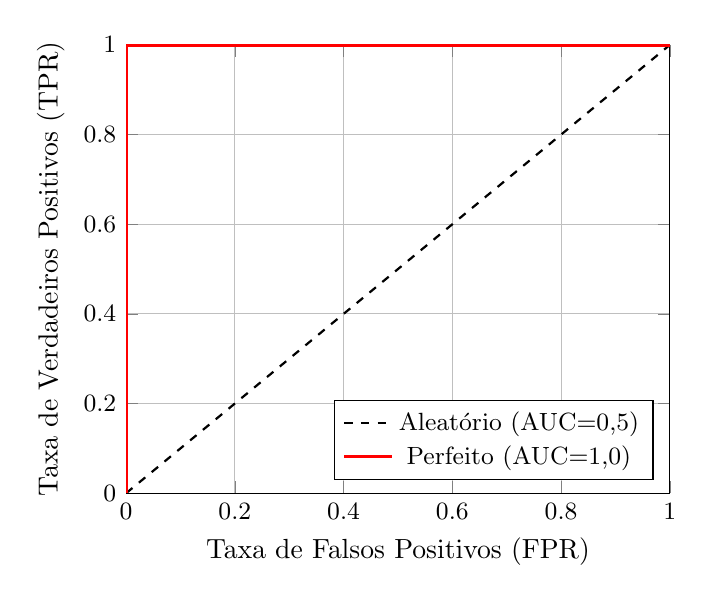
\begin{tikzpicture}
        \begin{axis}[
            width=0.7\textwidth,
            height=0.6\textwidth,
            grid=both,
            xlabel={Taxa de Falsos Positivos (FPR)},
            ylabel={Taxa de Verdadeiros Positivos (TPR)},
            xmin=0, xmax=1,
            ymin=0, ymax=1,
            legend pos=south east,
            legend style={font=\small},
            tick label style={font=\small}
        ]

        % Linha do classificador aleatório
        \addplot[domain=0:1, dashed, thick, color=black] {x};
        \addlegendentry{Aleatório (AUC=0,5)}

        % Curva ROC do Classificador Perfeito
        \addplot[color=red, very thick] coordinates {
            (0,0)  % Inicia
            (0,1)  % Sobe verticalmente até TPR=1, mantendo FPR=0
            (1,1)  % Segue horizontalmente até o fim, mantendo TPR=1
        };
        \addlegendentry{Perfeito (AUC=1,0)}

        \end{axis}
        
    \end{tikzpicture}
    \label{fig:roc_perfect}
    \legend{Fonte: Elaborado pelo autor.}
\end{figure}

Já a curva PR, Precisão vs \textit{Recall} representa a precisão em função do \textit{recall}. Na figura Figure~\ref{fig:roc_perfect},
é ilustrada a curva PR de um classificador perfeito.

\pgfplotsset{compat=1.18}

\begin{figure}[H]
    \centering
    \caption{Curva Precisão–Recall de um Classificador Perfeito: Comparação com Baseline.}
    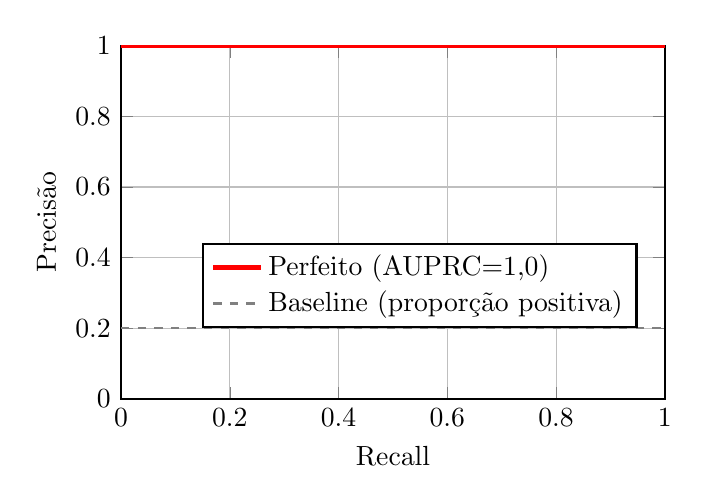
\begin{tikzpicture}
        \begin{axis}[
            width=0.7\textwidth,
            height=0.5\textwidth,
            xlabel={Recall},
            ylabel={Precisão},
            xmin=0, xmax=1,
            ymin=0, ymax=1,
            grid=major,
            legend style={at={(0.95,0.2)},anchor=south east},
            legend cell align={left},
            thick
        ]
        
        % Curva PR do Classificador Perfeito
        \addplot[color=red, ultra thick] coordinates {
            (0.0, 1.0)  % Precisão = 1, Recall = 0
            (1.0, 1.0)  % Precisão = 1, Recall = 1
        };
        \addlegendentry{Perfeito (AUPRC=1,0)}

        % Linha base (baseline) - Mantida como exemplo
        \addplot[dashed, color=gray] coordinates {
            (0,0.2) (1,0.2)
        };
        \addlegendentry{Baseline (proporção positiva)}
        \end{axis}
    \end{tikzpicture}
    
    \label{fig:pr_curve_perfect}
    \legend{Fonte: Elaborado pelo autor.}
\end{figure}


Na figura \ref{fig:pr_curve_perfect} representa uma curva PR genérica, a curva mostra a precisão em função do \textit{recall}. Como ilustrado,
conforme aumenta-se o \textit{recall}, há uma diminuição da precisão e vice-versa; representado o \textit{trade-off}. O AP é a área do gráfico; quanto
maior, melhor. Um modelo aleatório teria um AP igual a frequência da classe positiva.

A matriz de confusão, por fim, fornece uma representação tabular dos acertos e erros do modelo, como exemplificado na Tabela~\ref{tab:matriz_confusao}.

\begin{table}[H]
\centering
\caption{Exemplo de matriz de confusão binária}
\label{tab:matriz_confusao}
\begin{tabular}{|c|c|c|}
\hline
\multirow{2}{*}{\textbf{Classe Verdadeira}} & \multicolumn{2}{c|}{\textbf{Classe Predita}} \\ \cline{2-3} 
 & Positiva & Negativa \\ \hline
Positiva & TP & FN \\ \hline
Negativa & FP & TN \\ \hline
\end{tabular}
\legend{Fonte: Elaborado pelo autor.}
\end{table}

Essas métricas em conjunto permitem avaliar não apenas a proporção global de acertos, mas também a capacidade do modelo em detectar corretamente arritmias, aspecto essencial em aplicações médicas.

\section{Tipos de redes usadas}
\label{sec:tipo_redes}

Inicialmente, foram escolhidas redes neurais recorrentes (RNNs) e seus subtipos, como LSTM e GRU. Segundo \citeonline{james2023}, esse tipo de rede apresenta grande potencial para lidar com dados sequenciais, como no processamento de linguagem natural, previsão de preços e outros tipos de séries temporais. Como o componente temporal é relevante para o diagnóstico das arritmias, optou-se por esse tipo de modelo.

Além das RNNs, foram utilizadas redes neurais convolucionais (CNNs), conhecidas por sua habilidade em reconhecer padrões em diferentes domínios \citeonline{james2023}. Em particular, CNNs unidimensionais (1D-CNNs) têm se mostrado eficazes na análise de sinais fisiológicos, sendo amplamente aplicadas à classificação de ECG \cite{narotamo2024}.

A motivação para essa combinação está na complementaridade entre os modelos: enquanto as RNNs são eficazes na captura de dependências temporais, as CNNs se destacam na identificação de características morfológicas do sinal.

\section{Pré-processamento e entrada para os modelos}
\label{sec:pre_process}

Antes de usar o sinal do ECG como entrada, ele precisou passar por uma etapa de pré-processamento que consistiu em uma limpeza de ruídos e segmentação.
Para a diminuição do ruído, foi utilizando um filtro passa-alta de ordem 5 de 0,5 hz, seguido por uma filtragem de linha de energia de 60hz. 
Isso foi importante para remover ruídos musculares e ruídos oriundos da alimentação dos aparelhos. 

Em seguida, os batimentos foram segmentados em batimentos individuais. Nas duas etapas foram utilizadas a biblioteca NeuroKit2 \cite{Makowski2021neurokit}

O objetivo do trabalho é a classificação de batimentos cardíacos em duas classes: normais e arritmia ventricular. 
Para isso, os modelos recebem uma sequência de 16 batimentos e realizam a classificação do último batimento da sequência. 
Cada sequência é composta exclusivamente por batimentos de um único paciente

Tanto as CNNs quanto as RNNs recebem como entrada uma matriz tridimensional com a seguinte estrutura: $(\text{tamanho do batch}, \text{tamanho da sequência}, \text{número de features})$.

Para otimização do processo de treinamento, foram utilizados os mecanismos de \textit{early stopping} e \textit{reduce on plateau}, responsáveis por limitar o número de épocas e ajustar dinamicamente a taxa de aprendizagem, respectivamente.

\section{Arquiteturas}
\label{sec:modelos}

Foram testadas dois tipos de arquiteturas, uma é o uso de RNNs puras e a outra é uma arquitetura híbrida com CNNs. 

A primeira arquitetura de pura é composta por três camadas de GRUs com 256 unidades ocultas. Essa arquitetura foi utilizada em \citeonline{narotamo2024}, onde obteve o melhor desempenho. 
A diferença é que nesse trabalho, além da rede receber o sinal do ECG, ela também recebeu os intervalos RRs pré e pós:


\begin{figure}[H]
  \centering
  \caption{Arquitetura GRU pura.}
  \begin{tikzpicture}[node distance=1.5cm, every node/.style={draw, rounded corners, minimum width=2.8cm, minimum height=1cm, align=center}]

\node (input){Entrada ECG e features};
\node [below=of input](gru_1){GRU};
\node [below=of gru_1](gru_2){GRU};
\node [below=of gru_2](gru_3){GRU};
\node [below=of gru_3](saida){Classificação final};

%conexões:

\draw[->](input) -- (gru_1);
\draw[->](gru_1) -- (gru_2);
\draw[->](gru_2) -- (gru_3);
\draw[->](gru_3) -- (saida);
\end{tikzpicture}
 % insere o tikzpicture puro
  \label{fig:gru_pura}
  \legend{Fonte: Elaborado pelo autor.}
\end{figure}

A segunda rede é uma híbrida de CNN com GRU:

\begin{figure}[H]
  \centering
  \caption{Arquitetura híbrida CNN e GRU.}
  \begin{tikzpicture}[node distance=1.5cm, every node/.style={draw, rounded corners, minimum width=2.8cm, minimum height=1cm, align=center}]

% Entradas
\node (morf) {Entrada Morfológica (ECG)};
\node[right=of morf] (ritmo) {Entrada features};

%blocos de redes neurais:
\node[below=1.5cm of morf] (cnn) {Bloco CNN \\ (extração morfológica)};

% Combinação
\node[below=1.5cm of cnn, xshift=2.5cm] (fusion) {Combinação das Saídas};

% Bloco RNN
\node[below=of fusion] (rnn) {Bloco GRU \\ (padrões temporais)};

%saída
\node[below=of rnn] (saida) {Classificação Final};

%conexões
\draw[->](morf) -- (cnn);
\draw[->](cnn) -- ++ (fusion);
\draw[->](ritmo) -- ++ (fusion);
\draw[->](fusion) -- (rnn);
\draw[->](rnn) -- (saida);

\end{tikzpicture}

 % insere o tikzpicture puro
  \label{fig:cnn_gru}
  \legend{Fonte: Elaborado pelo autor.}
\end{figure}

O bloco de CNN precisou ser aplicado em cada batimento dentro da sequência. Trata-se de duas camadas de CNN com 32 e 64 filtros respectivamente e cada 
uma seguida por uma camada de \textit{batch normalization} e \textit{global max pooling} para evitar sobre ajuste e reduzir as \textit{features} respectivamente.

Enquanto que a rede da figura \ref{fig:gru_pura} recebeu o ECG concatenado com as \textit{features}, a rede híbrida as recebeu separadas, sendo conectadas após o processamento
das CNNs.
